\subsection{Specification of Boundary Conditions for the Input Geometry}
\label{sec: GeomCreation}

As pointed out in the \ref{sec:CADbackg}, STEP and IGES files can store color information for each face. This is the attribute that is used to specify the identity of the face, and can be modified using standard CAD design software such as FreeCAD (see \cite{FreeCAD}). When analysing a structural problem, a designer typically needs to provide information on up to five parameters:

\begin{itemize}
	\item \textbf{Optimized domain}: This refers to the main geometry that needs to be optimised. These faces are simply colored absolute white, i.e. $(255, 255, 255)$.
	\item \textbf{Fixture faces}: These faces of the geometry are meant to be fixed in space, and undergo zero displacement. These faces are colored absolute red, i.e. if the color space of red ranges in {$[0, 255]$}, then the face is assigned the extremum $255$. The blue and green color components are set to $0$. Thus, the color array is set to $(255, 0, 0)$. These are also stored in the file holding the optimized domain.
	\item \textbf{Load faces and load value}: These faces bear the forces acting on the body. Loads are three-dimensional, and can take both positive and negative values depending on their direction. To accommodate all possibilities, each color component (i.e. red, blue and green) is assigned a direction ($x$, $y$, and $z$). The range $(0, 255)$ is split in two: $(0, 127]$ representing the negative force range and $[128, 255)$ representing the positive force range. The color is then offset by $-127$. 

Internally, OpenCascade transforms the colors from range $(0, 255)$ to $(0,1)$ which we then shift to $(-0.5, 0.5)$. Of course, force values may also lie outside this range. The user then needs to scale the required force to fit in the color range, and provide a scaling factor as an input.

For example, to assign a force value of $(-200.5, 172.0, -10.75)$:

\begin{table}[h!]
	\begin{center}
		\caption{Fitting a force value to a color}
		\label{LoadFaceExample}
		\begin{tabular}{cccc}
			\toprule
			{\small Original vector} & {\small Scaling factor} & {\small OpenCascade values} & {\small Final color}\\
			\midrule
			$-200.5$ & $401$ & $-0.49$ & $001$\\
			$+172.0$ & $401$ & $+0.43$ & $235$\\
			$-10.75$ & $401$ & $-0.03$ & $120$\\
			\bottomrule
		\end{tabular}
	\end{center}
\end{table}

The load faces are given in a specified input file such that for example inner loads can be described.

	\item \textbf{Non-changing geometry}: Sometimes, certain parts of the geometry cannot accommodate changes. This could be for several reasons, for example, due to compatibility issues with other components. To define the geometry accurately and independently of the main geometry, it is provided in a distinguished file.% These faces are marked with absolute green, i.e. $(0, 255, 0)$.
	\item \textbf{Solution limits:} The designer may be interested in restricting the solution to a certain region in space. This can be done by creating CAD geometry enclosing this region. Since this region could be different from the main geometry, it is specified through an additional file.
\end{itemize}

\autoref{fig: CADTopInputFiles} illustrates in more detail how the inputs needs to be defined to describe the constraint geometry. 

%The user must save the CAD file in both STEP and IGES formats. This is necessary due to some issues with the face extraction process in OpenCascade - the IGES format allows for proper face extraction, but color detection works only for the STEP format. Also, the files should be saved in the same directory, and have the same name.
\begin{figure}
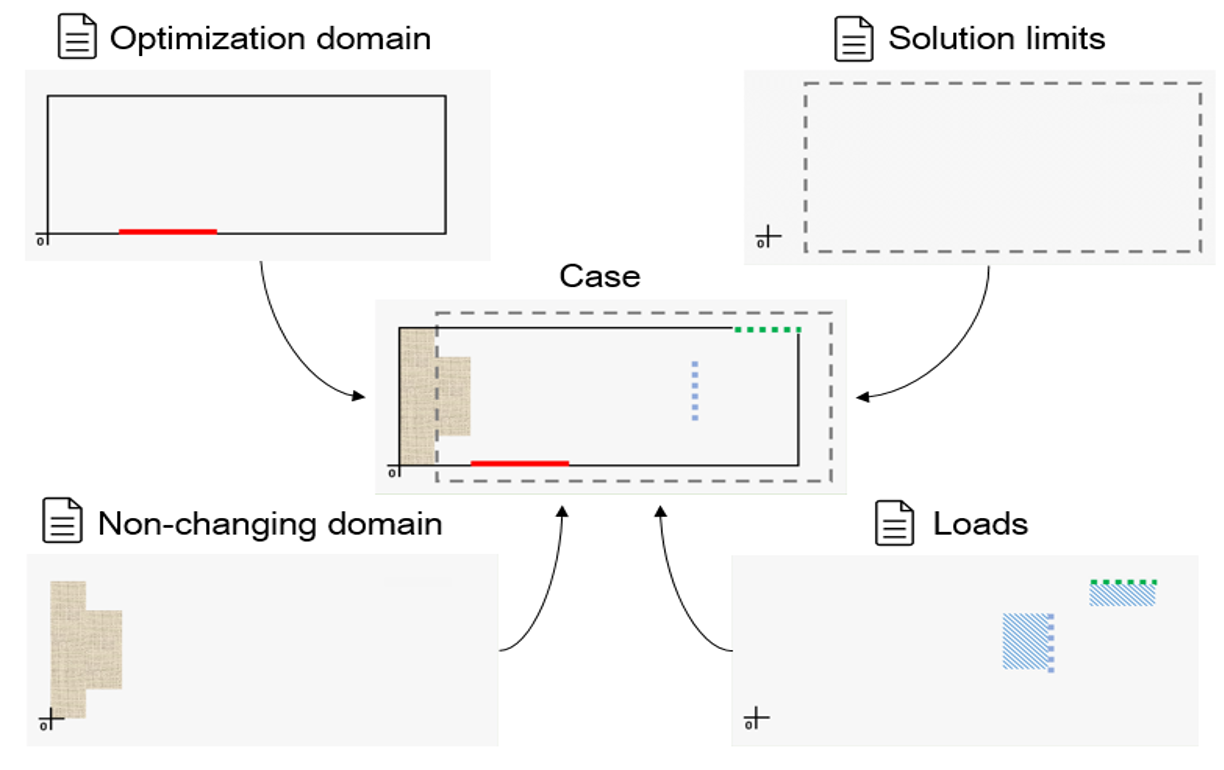
\includegraphics[width=\textwidth]{Pictures/four_files.png}
\caption{Assume the input file is called \texttt{input{\_}file}. The optimization domain(top left) describes the main geometry and has to be provided in files \texttt{input{\_}file.step} and \texttt{input{\_}file.iges}. Here, files of type \texttt{.step} store the structural description while \texttt{.iges} hold the color information. Also the fixture faces are stored in these files. The solution limits are given in a file \texttt{input{\_}file{\_}toOptimize.step} (top right). Similarly, the non-changing domain stored as \texttt{input{\_}file{\_}Fixed.step} (bottom left). Finally, also the loads are specified in a seperate input file named \texttt{input{\_}file{\_}load.step} (bottom right).}
\label{fig: CADTopInputFiles}
\end{figure}
